\thispagestyle{firststyle}
\large

\begin{center}
    {\LARGE\bfseries Решения заключительного отбора Сириус 7 класс 2026 год.}\\[2mm]
\end{center}

\problem{1}
Дан клетчатый прямоугольник $2\times 3$. Cколько существует способов расставить цифры от $1$ до $6$ так, чтобы соседние по стороне цифры были взаимно простыми.

\textit{Решение.}
Будем смотреть не на хорошие соседства, а на запрещённые. Среди чисел $1,2,3,4,5,6$ невзаимно простые пары такие:
\[
(2,4),\quad (2,6),\quad (3,6),\quad (4,6).
\]
Значит, число $6$ не может стоять рядом с $2,3,4$. Рядом с $6$ могут стоять только $1$ и $5$.

В прямоугольнике $2\times3$ есть четыре угловые клетки степени $2$ и две средние клетки степени $3$. Если поставить $6$ в среднюю клетку, у неё будет три соседа, но безопасных соседей для $6$ только два: $1$ и $5$. Поэтому $6$ обязательно стоит в углу.

\begin{center}
\begin{tikzpicture}[scale=0.95, every node/.style={font=\large}]
    \draw[step=1, line width=0.6pt] (0,0) grid (3,2);
    \node at (0.5,1.5) {$6$};
    \node[fill=green!15, rounded corners=1pt, inner sep=2pt] at (1.5,1.5) {$1/5$};
    \node[fill=green!15, rounded corners=1pt, inner sep=2pt] at (0.5,0.5) {$1/5$};
    \node at (2.5,1.5) {$\ast$};
    \node at (1.5,0.5) {$\ast$};
    \node at (2.5,0.5) {$\ast$};
    \draw[-{Latex[length=2mm]}, thick, blue!70!black] (0.42,1.5) -- (1.5,1.5);
    \draw[-{Latex[length=2mm]}, thick, blue!70!black] (0.42,1.5) -- (0.42,0.42);
\end{tikzpicture}
\qquad
\begin{tikzpicture}[scale=0.95, every node/.style={font=\large}]
    \draw[step=1, line width=0.6pt] (0,0) grid (3,2);
    \node[gray] at (0.5,1.5) {$6$};
    \node[gray] at (1.5,1.5) {$1/5$};
    \node[gray] at (0.5,0.5) {$1/5$};
    \node[fill=yellow!20, rounded corners=1pt, inner sep=2pt] at (2.5,1.5) {$2/4$};
    \node[fill=yellow!20, rounded corners=1pt, inner sep=2pt] at (1.5,0.5) {$2/4$};
    \node[fill=orange!20, rounded corners=1pt, inner sep=2pt] at (2.5,0.5) {$3$};
    \draw[-{Latex[length=2mm]}, thick, red!70!black] (2.5,0.5) -- (2.5,1.5);
    \draw[-{Latex[length=2mm]}, thick, red!70!black] (2.5,0.5) -- (1.5,0.5);
\end{tikzpicture}
\end{center}

Пусть $6$ уже стоит в углу. Тогда две соседние с ним клетки обязаны быть заняты числами $1$ и $5$. Это можно сделать $2$ способами.

Остаются три клетки и числа $2,3,4$. Эти три клетки образуют цепочку из трёх клеток. Числа $2$ и $4$ не могут быть соседями, значит, они должны стоять на концах цепочки, а число $3$ -- в середине. Концы для $2$ и $4$ можно выбрать $2$ способами.

Угол для числа $6$ можно выбрать $4$ способами. Поэтому всего
\[
4\cdot 2\cdot 2=16.
\]

\textit{Ответ: 16.}


\problem{2}
Сегодня возраст Ивана -- квадрат натурального числа, и $13$ лет назад его возраст тоже был квадратом натурального числа. Через сколько лет Ивану станет лет -- ближайший больший куб натурального числа?

\textit{Решение.}
Пусть сейчас Ивану $n^2$ лет, а $13$ лет назад ему было $m^2$ лет. Тогда
\[
n^2-m^2=13.
\]
Разложим левую часть:
\[
(n-m)(n+m)=13.
\]
Число $13$ простое, поэтому
\[
n-m=1,\qquad n+m=13.
\]
Отсюда $n=7$, $m=6$. Значит, сейчас Ивану $7^2=49$ лет, а $13$ лет назад ему было $6^2=36$ лет. Следующий куб натурального числа после $49$ -- это $4^3=64.$ Значит, Ивану станет $64$ года через $64-49=15$ лет.

\textit{Ответ: 15}

\problem{3}
У Винни-Пуха есть чашечные весы и погреб с банками мёда, вес которых $1,2,3,\ldots,15$ кг. Винни-Пух может взять две банки. Если их вес равен, он съедает весь мёд. Иначе он выливает из лёгкой банки на левую чашу весь мёд, а на правую чашу из второй банки выливает столько мёда, пока не будет равенство. Остаток мёда он кладёт обратно в погреб, а мёд с весов съедает. Сколько максимум мёда у него может остаться?

\begin{center}
\begin{tikzpicture}[scale=0.55, every node/.style={font=\small}]
    \newcommand{\jar}[3]{
        \begin{scope}[shift={(#1,#2)}]
            \draw[rounded corners=2pt, fill=yellow!18] (0,0) rectangle (0.65,0.85);
            \draw[fill=orange!35] (0.06,0.08) rectangle (0.59,0.52);
            \draw[fill=gray!20] (0.12,0.85) rectangle (0.53,1.03);
            \node at (0.325,-0.25) {#3};
        \end{scope}
    }
    \foreach \w [count=\i from 0] in {1,2,3,4,5,6,7,8} {\jar{\i*0.95}{0}{\w}}
    \foreach \w [count=\i from 0] in {9,10,11,12,13,14,15} {\jar{\i*0.95+0.5}{-1.55}{\w}}
\end{tikzpicture}
\end{center}


\textit{Решение.}
Если Винни-Пух берёт банки веса $x$ и $y$, где $x\le y$, то он съедает $2x$ кг мёда, а обратно кладёт $y-x$ кг. Значит, операция заменяет пару чисел $x,y$ на число $|x-y|$; если $x=y$, обе банки исчезают.

Сначала докажем верхнюю оценку. Общий вес мёда уменьшается на $2x$, то есть всегда на чётное число. Поэтому чётность общего оставшегося веса сохраняется. Изначально
\[
1+2+\ldots+15=120,
\]
то есть общий вес чётный.

Кроме того, вес любой банки никогда не увеличивается: вместо двух банок остаётся разность их весов, а она меньше большего из двух весов. Значит, в конце не может остаться банка тяжелее $15$ кг. Если процесс закончился и осталась одна банка, её вес должен быть чётным, потому что общий оставшийся вес чётный. Поэтому вес последней банки не может быть равен $15$; значит, он не превосходит $14$.

Осталось показать, что $14$ кг действительно можно оставить. Будем не трогать банку $14$ кг, а остальные банки уничтожим следующими операциями. В таблице запись $a,b\to c$ означает, что из банок $a$ и $b$ остаётся банка $|a-b|=c$; запись $a,a\to0$ означает, что две равные банки съедаются полностью.

\begin{center}
\begin{tabular}{c>{\centering\arraybackslash}p{8.5cm}}
\toprule
Шаг & Операция \\
\midrule
1 & $5,6\to1$ \\
2 & $1,7\to6$ \quad\textit{здесь берём новую банку $1$ кг} \\
3 & $4,8\to4$ \\
4 & $6,4\to2$ \quad\textit{берём новые банки $6$ кг и $4$ кг} \\
5 & $2,9\to7$ \quad\textit{берём новую банку $2$ кг} \\
6 & $3,10\to7$ \\
7 & $7,7\to0$ \\
8 & $1,12\to11$ \quad\textit{теперь берём исходную банку $1$ кг} \\
9 & $11,11\to0$ \\
10 & $2,15\to13$ \quad\textit{теперь берём исходную банку $2$ кг} \\
11 & $13,13\to0$ \\
\bottomrule
\end{tabular}
\end{center}

После этих действий все банки, кроме банки $14$ кг, исчезли. Значит, $14$ кг можно оставить, а больше оставить нельзя.

\textit{Ответ: 14.}


\problem{4}
Дан прямоугольный треугольник $ABC$, угол $C$ -- прямой. Из угла $A$ проведена биссектриса $AQ$ к стороне $BC$. Из угла $B$ проведена биссектриса $BP$ к стороне $AC$. Точки $N$ и $M$ -- проекции точек $P$ и $Q$ соответственно на сторону $AB$. Найдите градусную меру угла $MCN$.

\textit{Решение.}

Пусть $\angle A = 2\alpha$, $\angle B = 2\beta$. Тогда $\angle BAQ = \angle QAC = \alpha$ и $\angle CBP = \angle PBA = \beta$. Заметим, что треугольник $PNA$ прямоугольный с острым углом $2\alpha$. Значит вторй острый угол $\angle NPA = 2\beta$. Аналогично $\angle BQM = 2\alpha$. Биссектриса это геометрическое место точек равноудаленных от сторон угла, а значит $CP = CN$. Значит углы $\angle NCP$ и $\angle  PNC$ равны и по теореме о смежном угле в сумме дают $2\beta$. Значит каждый из них по $\beta$. Аналогично каждый из углов $\angle QCM$ и $\angle QMC$ по $\alpha$. Тогда $\angle MCN = \angle BCA - (\angle QCM + \angle NCP) = 90^{\circ} - (\alpha + \beta) = 45.$

\begin{figure}
    \centering
    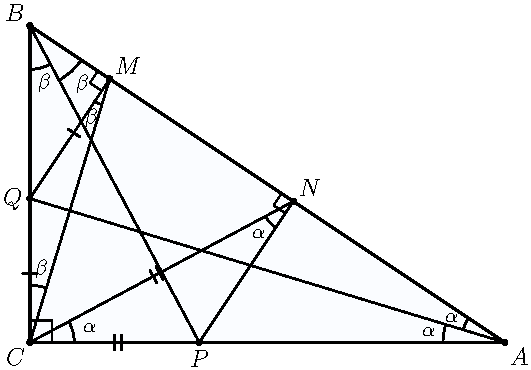
\includegraphics[width=0.5\linewidth]{ЭлМШ 2025-2026/разбор Сириуса/7/triangle_angle.pdf}
    \caption{Enter Caption}
    \label{fig:placeholder}
\end{figure}

\textit{Ответ: 45.}


\problem{5}
Дан квадрат $8\times8$. Петя закрашивает $n$ клеток этой доски. Вася может взять любой квадрат $2\times2$ и, если в нём закрашено $3$ клетки, закрасить оставшуюся. При каком наименьшем $n$ как бы ни раскрасил доску Петя, Вася всегда может полностью докрасить оставшуюся часть доски?

\textit{Решение.}
Будем смотреть на незакрашенные клетки. Вася может закрасить незакрашенную клетку тогда и только тогда, когда она является единственной незакрашенной клеткой в некотором квадрате $2\times2$.

Назовём множество незакрашенных клеток \textit{устойчивым}, если в каждом квадрате $2\times2$ находится либо $0$, либо хотя бы $2$ клетки этого множества. Если после всех возможных ходов Васи что-то осталось незакрашенным, то оставшиеся клетки образуют непустое устойчивое множество.

\textit{Лемма.}
Любое непустое устойчивое множество клеток на доске $8\times8$ содержит хотя бы $8$ клеток.
\begin{proof}
    Если оно имеет клетку в каждой из $8$ строк, то всё ясно: клеток хотя бы $8$. Иначе существует непустая строка, соседняя с пустой строкой. Рассмотрим эту непустую строку и любую пару соседних клеток в ней. Вместе с двумя клетками соседней пустой строки они образуют квадрат $2\times2$. В этом квадрате не может быть ровно одной клетки нашего устойчивого множества. Значит, в выбранной строке каждые две соседние клетки либо обе принадлежат множеству, либо обе не принадлежат. Поэтому вся строка устроена одинаково. Раз она непустая, она целиком принадлежит устойчивому множеству, то есть содержит $8$ клеток.
\end{proof}

Итак, непустое устойчивое множество всегда имеет размер хотя бы $8$.

Теперь если Петя закрасил $57$ клеток, то незакрашенных осталось только $7$. Непустого устойчивого множества среди них быть не может. Значит, процесс Васи не может остановиться раньше полной закраски доски; Вася обязательно докрасит всё.

Осталось показать, что $56$ клеток недостаточно. Петя может закрасить все клетки, кроме одной целой строки. Тогда в любом квадрате $2\times2$, пересекающем эту строку, незакрашены ровно две клетки, а не одна. Поэтому Вася не сможет сделать ни одного хода, который закрасил бы клетку этой строки.

\begin{center}
\begin{tikzpicture}[scale=0.47]
    \fill[gray!35] (0,0) rectangle (8,8);
    \fill[white] (0,3) rectangle (8,4);
    \draw[step=1, line width=0.45pt] (0,0) grid (8,8);
    \node[below] at (4,0) {Пример, почему $56$ клеток недостаточно};
\end{tikzpicture}
\end{center}

\textit{Ответ: 57.}

\section*{Задача 6}
\textbf{Условие.} Полина и Виктория забирают конфеты из непустых корзин. Корзины стоят по кругу, всего их $30$. Суммарно в корзинах $1000$ конфет. Полина за один ход забирает конфеты из двух соседних непустых корзин, а Виктория забирает из любой корзины, соседней с пустой. Докажите, что Полина может забрать $667$ конфет.

\textit{Решение.}
Пронумеруем корзины по кругу числами $1,2,\ldots,30$. Разобьём их на три класса по остаткам номеров при делении на $3$:
\[
1,4,7,\ldots,28;\qquad
2,5,8,\ldots,29;\qquad
3,6,9,\ldots,30.
\]
Суммарно во всех корзинах $1000$ конфет, поэтому в одном из этих трёх классов лежит не более
\[
\frac{1000}{3}<334
\]
конфет. Так как число конфет целое, в этом классе не более $333$ конфет. Назовём корзины этого класса красными.

Между любыми двумя соседними красными корзинами стоят ровно две некрасные соседние корзины. Полина будет забирать именно такие пары некрасных корзин, а Виктории будет оставлять красные корзины.

Опишем стратегию. Первым ходом Полина забирает любую пару соседних некрасных корзин, стоящую между двумя красными. После этого пустой участок на круге граничит с двумя красными корзинами, поэтому Виктория вынуждена взять одну из этих красных корзин.

Дальше Полина действует так: если Виктория только что взяла красную корзину на одном конце пустого участка, то Полина следующим ходом берёт две некрасные соседние корзины, которые идут сразу за этой красной корзиной. После хода Полины пустой участок снова граничит с красными корзинами. Значит, Виктория снова вынуждена брать красную корзину.

Так продолжается, пока корзины не закончатся. В итоге Виктория заберёт только красные корзины, а Полина -- все остальные. В красных корзинах было не больше $333$ конфет, значит, Полина заберёт не меньше
\[
1000-333=667
\]
конфет.